Forsøget med LCR-kredsløbet afbillede, hvordan spændingen er afhængig af hvilken frekvens, der benyttes. Samtidig svinger den samlede impedans i kredsløbet og ud fra det, kan strømmen beregnes for kredsløbet. Ud fra dette viser det sig, at strømstyrken også varierer i forhold til frekvensen, hvor strømmen når maksimum ved systemets resonante frekvens. Her er modstanden afgørende for, hvordan strømstyrken opfører sig ved forskellige frekvenser. Ved en lav modstand i systemet vil strømstyrken ved den resonante frekvens være meget høj i forhold til andre frekvenser, mens en stor modstand vil mindske udslaget. Til gengæld vil en stor modstand forstørre frekvensområdet, som strømstyrken vil toppe ved.

\begin{figure}[H]
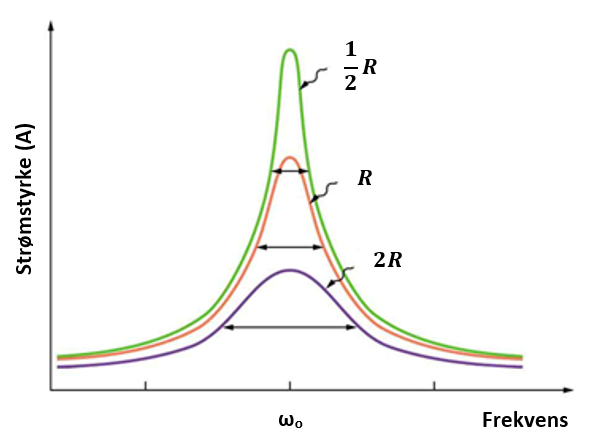
\includegraphics[scale=0.5]{Vildledning/Schematics/Resonanskurver}
\end{figure}

Graf X viser tre forskellige grafer over strømstyrken for systemet i forhols til frekvensen. Forskellen på de tre funktioner er, at der er forskellige størrelse modstande til de tre kredsløb. Den grønne graf har en modstand på $\frac{1}{2} R$, hvor strømstyrken giver et stort udsving ved den resonante frekvens. Til gengæld er udsvinget meget smalt, så frekvensen skal ikke afvige meget fra den resonante frekvens, før strømstyrken falder kraftigt. Ved den orange funktion er modstanden i systemet fordoblet. Her foretager strømstyrken igen et stort udsving ved den resonante frekvens, men stadig mindre end den grønne funktion. Til gengæld er udsvinget fladet mere ud, hvorved der kan ske større afvigelser fra den resonante frekvens, uden strømstyrken falder meget. For den lilla funktion, hvor modstanden er på $2 R$, så er udsvinget for strømstyrken lav ved den resonante frekvens i forhold til de to andre funktioner. Derimod strækker grafens udsving sig over et stort frekvensområde.

Grafen viser, at den resonante frekvens vil være optimal for det største output. Herefter afbilleder funktionerne, at den samlede modstand for systemet er afgørende for, hvor stort et output systemet har, og hvor let det er at ramme et højt output. Hvis der skal benyttes en lav strømstyrke, vil det være optimalt at benytte en stor modstand i kredsløbet for at give et bredt frekvensspektrum til den ønskede strøm. Derimod kræver høje output, at modstanden er lavt, hvorved der opstår et stort udslag, men så skal der omhyggeligt korrigeres for den resonante frekvens.